\documentclass[10pt]{article}

\usepackage[letterpaper,margin=1in,headheight=14pt]{geometry}
\usepackage[T1]{fontenc}
\usepackage[utf8]{inputenc}
\usepackage{newtxtext,newtxmath}
\usepackage{microtype}
\usepackage{amsmath,bm}
\usepackage{booktabs}
\usepackage{multirow}
\usepackage{graphicx}
\usepackage{subcaption}
\usepackage[table]{xcolor}
\usepackage{tikz}
\usetikzlibrary{positioning,arrows.meta,fit,backgrounds,calc}
\usepackage[numbers,sort&compress]{natbib}
\usepackage{fancyhdr}
\usepackage{titlesec}
\usepackage[font=small,labelfont=bf,skip=4pt]{caption}
\usepackage[colorlinks=true,linkcolor=blue!50!black,citecolor=blue!50!black,urlcolor=blue!50!black]{hyperref}
\usepackage[capitalise,noabbrev]{cleveref}
\usepackage{enumitem}
\setlist{nosep,leftmargin=1.4em}

\graphicspath{{figures/}}
% Generated by paper/scripts/build_assets.py. Do not edit.
\newcommand{\StartLives}{937}
\newcommand{\StartRare}{0}
\newcommand{\StartSteps}{199{,}936}
\newcommand{\StartSpanning}{7}
\newcommand{\StartSpanningRare}{3}
\newcommand{\BenchSpanning}{9}
\newcommand{\BenchSpanningRare}{6}
\newcommand{\BenchSpanningShortest}{48}
\newcommand{\FirstHandoffBeside}{20{,}704}
\newcommand{\EarlyStoneBeside}{17}
\newcommand{\EarlyRareBeside}{0}
\newcommand{\BenchMTwoTwoFieldCraftLives}{441}
\newcommand{\BenchMTwoTwoFieldCraftActor}{357}
\newcommand{\BenchMTwoTwoFieldCraftHandoffs}{60}
\newcommand{\BenchMTwoTwoFieldCraftTeacherrare}{23}
\newcommand{\BenchMTwoTwoFieldCraftActorrare}{0}
\newcommand{\BenchMTwoTwoFieldCraftTeacherpct}{38}
\newcommand{\BenchMTwoTwoFieldCraftHeldstone}{3, 2, 2, 3, 4}
\newcommand{\BenchMTwoTwoFieldCraftHeldstonefinal}{4}
\newcommand{\BenchMTwoThreeUniformWindowLives}{440}
\newcommand{\BenchMTwoThreeUniformWindowActor}{319}
\newcommand{\BenchMTwoThreeUniformWindowHandoffs}{121}
\newcommand{\BenchMTwoThreeUniformWindowTeacherrare}{44}
\newcommand{\BenchMTwoThreeUniformWindowActorrare}{0}
\newcommand{\BenchMTwoThreeUniformWindowTeacherpct}{36}
\newcommand{\BenchMTwoThreeUniformWindowHeldstone}{1, 2, 3, 3, 6}
\newcommand{\BenchMTwoThreeUniformWindowHeldstonefinal}{6}
\newcommand{\BenchMTwoFourWalkHomeLives}{460}
\newcommand{\BenchMTwoFourWalkHomeActor}{347}
\newcommand{\BenchMTwoFourWalkHomeHandoffs}{113}
\newcommand{\BenchMTwoFourWalkHomeTeacherrare}{23}
\newcommand{\BenchMTwoFourWalkHomeActorrare}{0}
\newcommand{\BenchMTwoFourWalkHomeTeacherpct}{20}
\newcommand{\BenchMTwoFourWalkHomeHeldstone}{1, 4, 2, 3, 2}
\newcommand{\BenchMTwoFourWalkHomeHeldstonefinal}{2}
\newcommand{\FieldCells}{116{,}235}
\newcommand{\FieldBaseline}{53.8}
\newcommand{\FieldGrassCells}{62{,}533}
\newcommand{\FieldStoneCells}{13{,}702}
\newcommand{\FieldPathCells}{17{,}852}
\newcommand{\FieldCoalCells}{1{,}609}
\newcommand{\FieldIronCells}{796}
\newcommand{\FieldTableCells}{725}
\newcommand{\FieldFurnaceCells}{167}
\newcommand{\RoomInAnchoredSuccess}{124}
\newcommand{\RoomInAnchoredActor}{147}
\newcommand{\RoomInAnchoredTimeouts}{23}
\newcommand{\RoomInAnchoredMedian}{36}
\newcommand{\RoomInAnchoredLate}{30/37}
\newcommand{\RoomInUniformSuccess}{85}
\newcommand{\RoomInUniformActor}{110}
\newcommand{\RoomInUniformTimeouts}{25}
\newcommand{\RoomInUniformMedian}{42}
\newcommand{\RoomInUniformLate}{25/28}
\newcommand{\RoomOutAnchoredSuccess}{185}
\newcommand{\RoomOutAnchoredActor}{190}
\newcommand{\RoomOutAnchoredTimeouts}{5}
\newcommand{\RoomOutAnchoredMedian}{38}
\newcommand{\RoomOutAnchoredLate}{48/48}
\newcommand{\RoomOutUniformSuccess}{130}
\newcommand{\RoomOutUniformActor}{138}
\newcommand{\RoomOutUniformTimeouts}{8}
\newcommand{\RoomOutUniformMedian}{46}
\newcommand{\RoomOutUniformLate}{35/35}
\newcommand{\PriorMTwoTwoFieldCraftAccOne}{70}
\newcommand{\PriorMTwoTwoFieldCraftTableOne}{0.35}
\newcommand{\PriorMTwoTwoFieldCraftAccFive}{65}
\newcommand{\PriorMTwoTwoFieldCraftTableFive}{0.18}
\newcommand{\PriorMTwoTwoFieldCraftAccOneFive}{56}
\newcommand{\PriorMTwoTwoFieldCraftTableOneFive}{0.08}
\newcommand{\PriorMTwoThreeUniformWindowAccOne}{69}
\newcommand{\PriorMTwoThreeUniformWindowTableOne}{0.24}
\newcommand{\PriorMTwoThreeUniformWindowAccFive}{65}
\newcommand{\PriorMTwoThreeUniformWindowTableFive}{0.27}
\newcommand{\PriorMTwoThreeUniformWindowAccOneFive}{57}
\newcommand{\PriorMTwoThreeUniformWindowTableOneFive}{0.08}
\newcommand{\PriorMTwoFourWalkHomeAccOne}{69}
\newcommand{\PriorMTwoFourWalkHomeTableOne}{0.29}
\newcommand{\PriorMTwoFourWalkHomeAccFive}{66}
\newcommand{\PriorMTwoFourWalkHomeTableFive}{0.27}
\newcommand{\PriorMTwoFourWalkHomeAccOneFive}{60}
\newcommand{\PriorMTwoFourWalkHomeTableOneFive}{0.08}
\newcommand{\ExamplePostAcc}{63}
\newcommand{\ExamplePriorAcc}{13}
\newcommand{\ExamplePostTable}{0.00}


\newcommand{\zpost}{z^{\mathrm{post}}}
\newcommand{\zprior}{z^{\mathrm{prior}}}
\newcommand{\method}{\textsc{Prospect}}
\newcommand{\rareset}{\mathcal{R}}

% ------------------------------------------------------------------ preprint style
\titleformat{\section}{\large\bfseries}{\thesection}{0.6em}{}
\titleformat{\subsection}{\normalsize\bfseries}{\thesubsection}{0.6em}{}
\titlespacing*{\section}{0pt}{1.4ex plus .4ex minus .2ex}{0.8ex plus .2ex}
\titlespacing*{\subsection}{0pt}{1.1ex plus .3ex minus .2ex}{0.5ex plus .2ex}
\titlespacing*{\paragraph}{0pt}{0.8ex plus .3ex minus .2ex}{0.8em}

\newcommand{\preprintdate}{November 24, 2026}
\pagestyle{fancy}
\fancyhf{}
\fancyhead[L]{\small\scshape A preprint}
\fancyhead[R]{\small\scshape \preprintdate}
\fancyfoot[C]{\thepage}
\renewcommand{\headrulewidth}{0.4pt}
\fancypagestyle{firstpage}{\fancyhf{}\renewcommand{\headrulewidth}{0pt}\fancyfoot[C]{\thepage}}

\newcommand{\keywords}[1]{\par\vspace{0.6em}\noindent{\small\textbf{Keywords:} #1}}

\makeatletter
\renewcommand{\@maketitle}{%
  \newpage\null\vskip -1.5em
  \begin{center}
    {\hrule height 2pt}\vskip 0.9em
    {\LARGE\bfseries \@title\par}\vskip 0.7em
    {\hrule height 0.6pt}\vskip 1.4em
    {\large\lineskip .5em \begin{tabular}[t]{c}\@author\end{tabular}\par}
    \vskip 0.8em {\small\scshape A preprint \,$\cdot$\, \preprintdate}
  \end{center}\par\vskip 1.2em}
\makeatother

\title{Does a World Model Know Where the Station Is?\\Probing a Dreamer Agent's Latent State\\with a Symbolic Field Head}

\author{
  \textbf{Aarush Verma}\\
  Independent Researcher\\
  \href{mailto:Aarush.business26@gmail.com}{\texttt{Aarush.business26@gmail.com}}
}

\date{}

\begin{document}

\maketitle
\thispagestyle{firstpage}

\begin{abstract}
A world model trained to reconstruct pixels has no reason to encode the one small tile that a rare action depends on: the reconstruction loss is dominated by large, frequent content, and at common encoder strides a single latent cell is larger than that tile.
We study \method{}, a DreamerV3-style recurrent state-space model with a single decoder and a \emph{field head} that predicts a local symbolic map (a material and an object class for every cell around the agent) from the latent state.
The actor reads that predicted field during imagination; in every run reported here, it reads the environment's field on real steps, including evaluation.
We vary two training conditions that should matter if the field is the bottleneck: where the action-relevant tile sits relative to the field, and whether training windows over demonstrations are anchored on the rare action.
On Crafter, probed on \FieldCells{} cells, the field head reaches 72\% cell accuracy against a \FieldBaseline\% all-grass baseline, but assigns the crafting station a mean probability of only 0.13--0.16.
Across three matched 100k-step runs, the actor performs the rare craft unaided in exactly two training lives in each run and in none of 10 held-out lives at any checkpoint, while a demonstrator given control finishes it on 23/60, 44/121, and 23/114 handoffs.
In a controlled room where the station occupies exactly one encoder cell, the field head names the station with probability above 0.98, and the actor learns the rare action in all four conditions, including when the station is behind the agent and when windows are not anchored; anchoring changes when the actor acts (median successful episode 36--38 vs.\ 42--46 steps), not whether it does.
Each configuration is a single seed.
The pattern is consistent with the benchmark failure lying in what the latent names, since imagination is where the actor is trained, rather than in where the demonstration places the tile. The room differs from the benchmark in more than that one respect, and we do not claim it isolates the cause.
\end{abstract}

\section{Introduction}
\label{sec:intro}

An agent that plans or learns inside a model of its environment can only use what that model represents.
World models compress observations into a latent state from which future observations, rewards, and episode ends can be predicted. They then train a policy on imagined rollouts of that state rather than on the environment \citep{ha2018worldmodels,hafner2019planet,hafner2020dreamer}.
DreamerV3 \citep{hafner2023dreamerv3,hafner2025dreamerv3nature} made this recipe work across domains with fixed hyperparameters, and world models now range from interactive video simulators \citep{bruce2024genie,hafner2025dreamer4} to theory arguing that general agents must contain one \citep{richens2025general}.
What the latent state of a reconstruction-trained world model represents, however, is decided mostly by a pixel loss.
That loss weighs every pixel equally and is dominated by large, frequent regions of the frame; small task-critical elements can drop out of the reconstruction entirely \citep{burchi2024mudreamer}.
A decision that depends on one small tile, such as crafting next to a workstation, gives the reconstruction loss almost nothing to pay for.
Recent probing work shows that a model can predict well while encoding an incoherent picture of the world \citep{vafa2024evaluating,gonzalezlaiz2026limits}.
This raises a representation question that a return curve cannot answer: \emph{does the agent's learned state contain the fact its rare decision depends on?}

We study this question with \method{}, a recurrent state-space model (RSSM) in the DreamerV3 family with one addition: a \emph{field head}.
The field head reads the latent state and predicts a local symbolic map, with a material class and an object class in each cell around the agent.
The actor reads that map alongside the latent features.
Imagination has no environment state, so in imagination the actor reads the field head's prediction.
In every run reported here, the actor reads the environment's true map on real steps, including evaluation.
We repeat this split throughout because it bounds what the experiments can show.

The field head turns the question into a measurement: \emph{does the latent name the tile the action needs?}
We pair the probe with two training conditions that should matter if the answer is no.
The first is where the action-relevant tile sits relative to the field: inside it while the demonstrator approaches, or outside it.
The second is whether training windows sampled from demonstrations are anchored to end on the rare action, or are ordinary slices that usually miss it.
We run both conditions on Crafter \citep{hafner2022crafter} with a large model and in a small controlled room with a small model, and report the same measurements in both.
\Cref{fig:example} shows the central observation on one benchmark frame.

\begin{figure}[t]
  \centering
  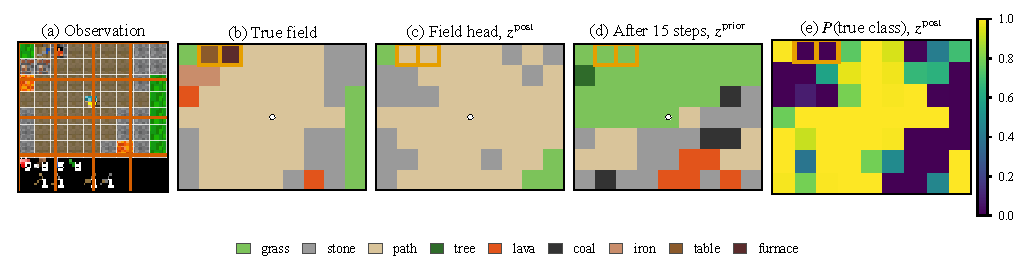
\includegraphics[width=\linewidth]{field_example.pdf}
  \caption{What the latent names on one benchmark frame (beside-resource anchored run, 100k steps). (a)~The $64\times64$ observation with Crafter's 7-pixel tiles (white) and the $16\times16$-pixel cells of the encoder's final feature map (orange): one latent cell spans more than two tiles in each direction. (b)~The true $9\times7$ field; the station tiles are outlined. (c)~The field head's prediction from the posterior latent: terrain is largely right (\ExamplePostAcc\% of cells), but the station is replaced by path, with probability \ExamplePostTable{} on the table tile. (d)~The same field after 15 imagined steps from the prior, the horizon on which the actor is trained: the map has drifted toward grass (\ExamplePriorAcc\% of cells). (e)~Probability of the true class per cell under the posterior. The frame is the probe frame with the most station cells in daylight; \cref{sec:latent} gives statistics over all \FieldCells{} probed cells.}
  \label{fig:example}
\end{figure}

\paragraph{Findings.}
\begin{itemize}
  \item \emph{On Crafter, the latent names terrain and not the station.} Probed on \FieldCells{} cells from eight demonstrator lives, the field head is correct on 72\% of cells, against \FieldBaseline\% for predicting the most common class everywhere. It assigns the true class a mean probability of 0.92 on grass, about 0.52 on stone, and 0.13--0.16 on the crafting table. After fifteen imagined steps, table recall is 0.08. All three 100k-step checkpoints agree (\cref{sec:latent}).
  \item \emph{On Crafter, the actor never performs the rare craft on its own,} in any of three matched runs, either in training lives or in 150 held-out lives. Neither condition changed this, although station placement did change how often the demonstrator finished the craft after a handoff: 23/60 and 44/121 when it placed the station beside the resource, against 23/113 when it walked back to it (\cref{sec:benchmark}).
  \item \emph{In the room, the latent names the station and the actor learns the rare action in all four conditions.} The station fills exactly one encoder cell. Success includes the condition in which the station is behind the agent and absent from the image at the moment of the action. Anchoring the training window shortened and tightened the successful episodes; it did not decide whether the action was learned (\cref{sec:room}).
  \item \emph{Three implementation pitfalls can invalidate this kind of study without any visible error} (\cref{app:identifiability,app:accounting}). A reconstruction path that skips the posterior lets pixel loss fall while the latent stays empty. A cloning loss averaged over uniform windows can reach zero while the rare action is absent from almost every window. Demonstrations injected on the environment instance used for collection let the agent's open episode inherit the demonstrator's achievements. In our logs, this produced every apparent unaided success of the rare action.
\end{itemize}

\paragraph{Scope.}
This is a study of what a world model's latent state represents and of when that limits a policy trained in imagination. It is not a benchmark result. We do not report a Crafter score as the method's score, because lives that the demonstrator finished would inflate it (\cref{app:accounting}). Every configuration is one seed, and held-out evaluations are ten lives. The room is deliberately easy, and its success is not evidence for the benchmark.

\paragraph{Organization.}
\Cref{sec:related} positions the work. \Cref{sec:method} defines \method{} without reference to either environment, and \cref{sec:setup} instantiates it. \Cref{sec:latent} reports what the latent names, \cref{sec:benchmark,sec:room} report the two conditions in each setting, and \cref{sec:discussion} states the limitations.

\section{Related work}
\label{sec:related}

Our question sits between three lines of work: model-based agents that act on a learned state, methods for asking what such a state represents, and the use of privileged information and demonstrations to shape it.
\citet{ding2025survey} survey world models along a similar divide, between models that build an internal representation of the world and models that predict its future to guide decisions; \method{} probes the first in service of the second.

\paragraph{World models and imagination.}
Learning a model of the environment and training behavior inside it goes back to Dyna \citep{sutton1991dyna} and was carried to pixels by \citet{ha2018worldmodels}.
PlaNet introduced the recurrent state-space model \citep{hafner2019planet}; Dreamer learned an actor and critic from imagined latent rollouts \citep{hafner2020dreamer}; DreamerV2 introduced categorical latents \citep{hafner2021dreamerv2}; and DreamerV3 made the recipe robust across domains with fixed hyperparameters \citep{hafner2023dreamerv3,hafner2025dreamerv3nature}.
Recent work extends the backbone with structured state-space memory \citep{samsami2024r2i}, transformers \citep{micheli2023iris,zhang2023storm}, and contrastive objectives over future latents \citep{burchi2025twister}.
It also scales world models toward interactive simulators: diffusion models of Atari and of a full first-person game \citep{alonso2024diamond,valevski2025gamengen}, foundation models of controllable environments learned from unlabeled video \citep{bruce2024genie}, and Dreamer~4, which trains a Minecraft agent entirely inside a video world model \citep{hafner2025dreamer4}.
A parallel line predicts in a learned or pretrained feature space without reconstructing pixels and plans there \citep{schrittwieser2020muzero,hansen2024tdmpc2,zhou2025dinowm,assran2025vjepa2}.
On the theory side, \citet{richens2025general} prove that any agent capable of generalizing across multi-step goal-directed tasks must have learned a predictive model of its environment.
\method{} keeps the DreamerV3 graph and adds a supervised head. The question we ask is what that graph's latent names, not how to raise its returns.

\paragraph{What reconstruction does and does not encode.}
Pixel reconstruction spends capacity on visually dominant but task-irrelevant content.
Proposed remedies include separating task-relevant from irrelevant factors \citep{fu2021tia}, replacing reconstruction with prototype or predictive objectives \citep{deng2022dreamerpro,burchi2024mudreamer}, and rebalancing the observation and reward losses \citep{ma2024harmonydream}.
\citet{burchi2024mudreamer} report that DreamerV3's reconstructions can drop task-critical elements when those elements are small.
DIAMOND argues the opposite direction, that compressing away visual detail can drop information that matters for control \citep{alonso2024diamond}.
On Craftax-Classic, a transformer world model improves markedly when its tokenizer encodes each 7-pixel tile separately rather than the frame as a whole \citep{dedieu2025improving}, which indicates that the alignment between tiles and model units matters for performance.
Our observation is narrower and complementary: at common encoder strides, the tile an action depends on can be smaller than one latent cell, and a supervised field head shows directly whether the latent states that tile's content.

\paragraph{Probing world models.}
Classifier probes are a standard way to ask whether a representation contains a variable \citep{alain2017probes}, with the caveat that an expressive probe can learn the task itself \citep{hewitt2019control}.
Probes on Atari state variables have been used to evaluate reinforcement-learning representations \citep{anand2019atariari}, and a sequence model trained only on game transcripts carries a probe-decodable board state \citep{li2023othello}.
\citet{li2025worldmodeldef} give operational criteria for saying that a network has learned a world model, based on a simple (e.g.\ linear) map from its internal state to a nontrivial image of the data-generating process.
Recent empirical work asks whether such representations are coherent: generative models that pass next-token and probe diagnostics can still recover incoherent world models \citep{vafa2024evaluating}; video generators that look realistic fail physical-reasoning tests \citep{motamed2026physicsiq}; and large video encoders represent physical variables in a distributed rather than factorized form \citep{joseph2026physics}.
For reinforcement-learning world models specifically, object positions and scores are linearly decodable from IRIS and DIAMOND on Atari \citep{zhang2026probing}, while DreamerV3, TD-MPC2, and a JEPA-style model can earn reward on simple control tasks without faithfully modeling the dynamics \citep{gonzalezlaiz2026limits}.
Our field head differs in two ways. It is trained jointly with the world model, so it measures what the latent is pushed to carry. It is also the quantity the actor consumes in imagination, so its failures bear directly on the policy.

\paragraph{Privileged information as a target or an input.}
Using information available only at training time goes back to learning using privileged information \citep{vapnik2009lupi}; in control, privileged state can train a critic while the actor sees observations \citep{pinto2018asymmetric}.
The closest prior work is the Informed POMDP, which trains a Dreamer world model to predict training-time information rather than observations and finds that this speeds learning \citep{lambrechts2024informed}. Its follow-up identifies a limitation in the privileged-information representations that this Informed Dreamer learns and replaces the prediction target with latent guidance \citep{lambrechts2026reinformed}.
Scaffolder uses privileged sensors to scaffold the world model, critic, and other training components of a policy deployed on target observations \citep{hu2024scaffolder}.
PIGDreamer aligns a DreamerV3 observation model with a privileged-state model and gives critics privileged access while the actor stays observation-only \citep{huang2025pigdreamer}; a related line reconstructs privileged simulator state in place of images \citep{krinner2025ssmwm}, and SkyDreamer uses an Informed-Dreamer decoder of privileged flight state for interpretability in vision-based drone racing \citep{verraest2025skydreamer}.
Training with a linear probe that decodes true world features into the recurrent state improves prediction and reduces open-loop drift \citep{zahorodnii2025probes}, which is the closest training recipe to our field head, though that probe is not consumed by a policy.
\method{} predicts a discrete egocentric map of the kind these works use as a training signal, and asks a question they do not: whether the latent names the specific tile a rare action needs, both in the posterior and during imagination.
On real steps in our runs the actor also receives the true field, which we treat as a limitation of the evaluation rather than a feature of the method.

\paragraph{Demonstrations inside an online loop.}
Large-scale video pretraining has produced agents for long-horizon crafting in Minecraft \citep{baker2022vpt}.
With learned world models, demonstrations have been used to pretrain and seed a TD-MPC agent \citep{hansen2023modem}, to learn stage-wise rewards, a policy, and a world model jointly for long-horizon manipulation \citep{escoriza2025demo3}, and to train a DreamerV3 world model while the actor still learns only in imagination \citep{staley2024wmhd}.
We did not find prior work that adds a cloning loss on scripted demonstrations to a Dreamer actor trained in imagination, which is what \method{} does.

\paragraph{Rare events in imagination and replay.}
Sampling replay to emphasize important sequences is common; Curious Replay prioritizes Dreamer's replay by novelty \citep{kauvar2023curious}.
Recent work instead steers the world model's imaginations themselves toward rare but high-impact outcomes, such as task failures, so that policies can be evaluated and improved against futures that nominal rollouts miss \citep{seo2026stressdream}.
Our anchored window is a simpler member of this family, applied to demonstrations rather than to imagined futures; on the benchmark it did not change the actor's behavior.

\paragraph{Crafter.}
Crafter evaluates 22 achievements in a procedurally generated survival world \citep{hafner2022crafter}, and Craftax reimplements and extends it for fast experimentation \citep{matthews2024craftax}.
Recent agents include a transformer world model that exceeds DreamerV3 and human performance on Craftax-Classic \citep{dedieu2025improving}, object-centric agents \citep{stanic2023crafterood}, and a suite of foundation models for behavior priors and instruction following in Crafter \citep{park2025crafterdojo}; Crafter is also part of a benchmark of agentic reasoning for large language and vision-language models \citep{paglieri2025balrog}.
\citet{stanic2023crafterood} found that strong baselines partly rely on reading the inventory display, a reminder that what a Crafter agent encodes is not obvious from its score.
We use Crafter as one benchmark for a measurement, not to compete on its score.

\section{\method{}}
\label{sec:method}

\method{} is a DreamerV3 world model \citep{hafner2023dreamerv3} with one extra prediction head and one change to how demonstrations enter replay.
\Cref{fig:architecture} shows the graph.
This section names no item from either environment; \cref{sec:setup} does.

\begin{figure}[t]
  \centering
  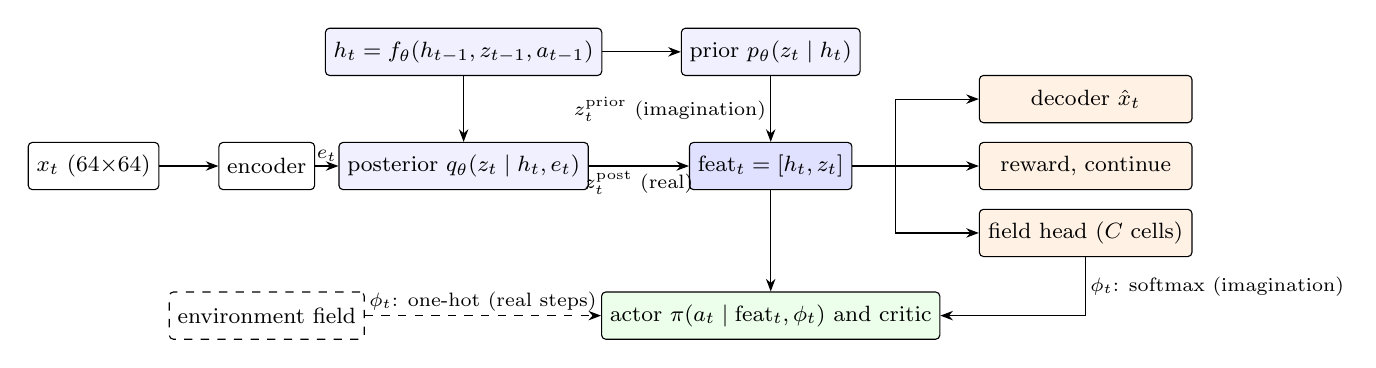
\begin{tikzpicture}[
    font=\footnotesize,
    >={Stealth[length=1.6mm]},
    box/.style={draw, rounded corners=1.5pt, minimum height=6mm, inner sep=3pt, align=center, fill=white},
    state/.style={box, fill=blue!6},
    head/.style={box, fill=orange!10, minimum width=27mm},
    act/.style={box, fill=green!8},
    lab/.style={font=\scriptsize, inner sep=1.5pt},
  ]
  \node[box]   (x)     at (0, 0)      {$x_t$ ($64{\times}64$)};
  \node[box]   (enc)   at (2.2, 0)    {encoder};
  \node[state] (post)  at (4.7, 0)    {posterior $q_\theta(z_t \mid h_t, e_t)$};
  \node[state] (h)     at (4.7, 1.45) {$h_t = f_\theta(h_{t-1}, z_{t-1}, a_{t-1})$};
  \node[state] (prior) at (8.6, 1.45) {prior $p_\theta(z_t \mid h_t)$};
  \node[box, fill=blue!12] (feat) at (8.6, 0) {$\mathrm{feat}_t = [h_t, z_t]$};
  \node[head]  (dec)   at (12.6, 0.85)  {decoder $\hat x_t$};
  \node[head]  (rc)    at (12.6, 0)     {reward, continue};
  \node[head]  (field) at (12.6, -0.85) {field head ($C$ cells)};
  \node[act]   (actor) at (8.6, -1.9) {actor $\pi(a_t \mid \mathrm{feat}_t, \phi_t)$ and critic};
  \node[box, dashed] (envf) at (2.2, -1.9) {environment field};

  \draw[->] (x) -- (enc);
  \draw[->] (enc) -- node[lab, above] {$e_t$} (post);
  \draw[->] (h) -- (post);
  \draw[->] (h) -- (prior);
  \draw[->] (post) -- node[lab, below] {$\zpost_t$ (real)} (feat);
  \draw[->] (prior) -- node[lab, left] {$\zprior_t$ (imagination)} (feat);
  \draw[->] (feat.east) -- ++(0.55,0) coordinate (fork) |- (dec.west);
  \draw[->] (fork) -- (rc.west);
  \draw[->] (fork) |- (field.west);
  \draw[->] (feat) -- (actor);
  \draw[->] (field.south) |- node[lab, pos=0.25, right] {$\phi_t$: softmax (imagination)} (actor.east);
  \draw[->, dashed] (envf) -- node[lab, above] {$\phi_t$: one-hot (real steps)} (actor);
\end{tikzpicture}

  \caption{\method{}. The encoder embedding $e_t$ enters only the posterior. One decoder and every head read $\mathrm{feat}_t=[h_t, z_t]$. The field head predicts a material and an object class for each of $C$ cells around the agent. The actor reads $\mathrm{feat}_t$ and a field $\phi_t$. In imagination, $\phi_t$ is the field head's softmax on $[h_t,\zprior_t]$. On real steps in every reported run, $\phi_t$ is the environment's field (dashed).}
  \label{fig:architecture}
\end{figure}

\subsection{World model}
\label{sec:method-wm}

Observations $x_t$ are $64\times64$ RGB frames.
A convolutional encoder maps each frame to an embedding $e_t$.
The RSSM \citep{hafner2019planet} carries a deterministic state $h_t$ and a stochastic state of 32 categorical variables with 32 classes each \citep{hafner2021dreamerv2}:
\begin{align}
  h_t &= f_\theta(h_{t-1}, z_{t-1}, a_{t-1}) && \text{(GRU \citep{cho2014gru})} \\
  \zpost_t &\sim q_\theta(z_t \mid h_t, e_t) && \text{(posterior, real data)} \\
  \zprior_t &\sim p_\theta(z_t \mid h_t) && \text{(prior, imagination)}
\end{align}
The posterior sees the current frame through $e_t$; the prior does not, and imagination rolls the prior alone.
Samples are drawn with straight-through gradients \citep{bengio2013estimating}.
A single decoder reconstructs $x_t$ from $\mathrm{feat}_t = [h_t, z_t]$ and from nothing else, together with reward and continuation heads on the same features.
The decoder input is a design constraint, not a default: any second reconstruction path that bypasses $\zpost_t$ gives the optimizer a way to lower pixel loss without putting information into the latent (\cref{app:bypass}).

The world-model loss is the DreamerV3 objective plus the field term below:
\begin{equation}
  \mathcal{L}_{\mathrm{wm}} = \mathcal{L}_{\mathrm{img}} + \mathcal{L}_{\mathrm{rew}} + \mathcal{L}_{\mathrm{cont}} + \lambda_{\mathrm{f}}\mathcal{L}_{\mathrm{field}}
  + \beta_{\mathrm{dyn}}\max\!\big(1, \mathrm{KL}[\mathrm{sg}(q)\,\|\,p]\big) + \beta_{\mathrm{rep}}\max\!\big(1, \mathrm{KL}[q\,\|\,\mathrm{sg}(p)]\big),
\end{equation}
where $\mathrm{sg}$ stops gradients and each KL, summed over the 32 latent variables, is floored at one nat as in DreamerV3 (the room model drops the floor on the dynamics term; \cref{app:hyper}).
$\mathcal{L}_{\mathrm{img}}$ is the squared error summed over pixels.

\subsection{Field head}
\label{sec:method-field}

The field is a $C$-cell grid around the agent, in the agent's frame.
Each cell $c$ has a material label $m_c \in \{1,\dots,M\}$ and an object label $o_c \in \{1,\dots,O\}$, read from the environment during training.
The field head is an MLP on $\mathrm{feat}_t$ that outputs $C$ categorical distributions over materials and $C$ over objects:
\begin{equation}
  \mathcal{L}_{\mathrm{field}} = \frac{1}{C}\sum_{c=1}^{C} \Big[ -\log p_\theta(m_c \mid \mathrm{feat}_t) - w(o_c) \log p_\theta(o_c \mid \mathrm{feat}_t) \Big],
\end{equation}
with $w(o_c)=4$ on cells that hold an object and 1 on empty cells, because almost every cell is empty.
The field is a training target for the latent.
It exists because the tile an action uses can be smaller than one cell of the encoder's final feature map, in which case reconstruction does not force the latent to say which material is on that tile (\cref{app:geometry}).

\subsection{What the actor reads}
\label{sec:method-actor}

The actor and critic are MLPs on $u_t = [\mathrm{feat}_t, \phi_t]$, where $\phi_t \in \mathbb{R}^{C(M+O)}$ is a field.
They are trained on imagined rollouts of horizon $H$ from every posterior state of a replay batch, with the DreamerV3 actor loss: REINFORCE on percentile-normalized $\lambda$-return advantages with an entropy bonus, and a two-hot critic with a slow target \citep{hafner2023dreamerv3}.
Imagination has no environment, so there $\phi_t$ is the softmax of the field head on $[h_t, \zprior_t]$.
We use the softmax rather than the argmax so that an uncertain cell reaches the actor as uncertain.
An environment can add further symbolic heads that the actor reads in the same way, and an action mask computed from them; the benchmark model has both (\cref{sec:setup-crafter}), and the room model has neither.

On a real step, $\phi_t$ can come from the same head on $[h_t, \zpost_t]$, or from the environment.
In every run in this paper it comes from the environment, as one-hot labels.
The policy that acts in the environment therefore sees the true field, while the policy gradient it learns from is computed on the predicted one.
If the field head does not name a tile in imagination, the actor receives no imagined return for the action that tile enables, even though it would see that tile when acting.

\subsection{Demonstrations in replay}
\label{sec:method-demos}

A scripted demonstrator produces episodes that are stored in the same replay as the actor's episodes, with a per-step demonstrator flag.
A fraction $\rho_T$ of the sequences in every batch are drawn from demonstrator episodes; the rest are drawn uniformly from all of replay.
The same batches train the world model and the actor-critic.

The actor additionally minimizes a behavior-cloning term on the posterior states of the batch \citep{pomerleau1988alvinn}:
\begin{equation}
  \mathcal{L}_{\mathrm{bc}} = \frac{\sum_{t} w_t \, \big[-\log \pi(a_t \mid u_t)\big]}{\sum_t w_t},
  \qquad
  w_t = \mathbb{1}[\text{demonstrator step}] \cdot \big(\kappa \text{ if } a_t \in \rareset \text{ else } 1\big),
\end{equation}
added to the actor loss with weight 1, where $\rareset$ is a small set of rare actions and $\kappa=8$.
The cloning term uses the same input $u_t$ the actor uses on real steps.

\subsection{The two conditions}
\label{sec:method-switches}

\paragraph{Window anchoring.}
A demonstrator episode is long, and the rare action occurs once or a few times near its end.
A window of length $L$ drawn uniformly from such an episode rarely contains it, and the cloning loss can approach zero while the rare action is absent from nearly every window (\cref{app:window}).
With probability $\rho_A$, a demonstrator draw is instead an \emph{anchored} window that ends on a step with $a_t\in\rareset$.
The \emph{uniform} condition sets $\rho_A=0$.
The weight $\kappa$ applies in both conditions whenever the rare action is in the window.

\paragraph{Tile placement.}
The demonstrator decides where the action-relevant tile is while it approaches and performs the rare action.
In the \emph{inside} condition it keeps that tile within the field the head is trained to name.
In the \emph{outside} condition the tile is outside the field for part of the demonstration.
How much of the demonstration that is depends on the environment's rules, and we give it for each setting in \cref{sec:setup}.

\section{Experimental setup}
\label{sec:setup}

We use one model family in two settings of very different difficulty.
\Cref{tab:hyper} in \cref{app:hyper} lists every hyperparameter.

\subsection{Benchmark: Crafter}
\label{sec:setup-crafter}

Crafter \citep{hafner2022crafter} renders a $64\times64$ image of the $9\times7$ tiles around the agent plus an inventory strip.
The field is that $9\times7$ grid ($C=63$), with $M=13$ material classes and $O=8$ object classes, read from the environment's semantic map.
The agent has 17 actions.
We use the reward version of the environment, \texttt{CrafterReward-v1}.

\paragraph{Rare action.}
The rare-action set $\rareset$ is the three actions that build or use a furnace: placing it, and crafting the iron pickaxe and the iron sword.
We report the iron pickaxe.
It needs wood, coal, and iron in the inventory and both a crafting table and a furnace (together, the \emph{station}) within one tile of the agent.
Under Crafter's rules, that three-by-three neighborhood always lies inside the $9\times7$ field, so at the moment of the craft the station is inside the field in every run.

\paragraph{Model and schedule.}
The world model is the DreamerV3 XL configuration as we implemented it: convolutional channels (96, 192, 384, 768) with two residual blocks per stage, a 4096-unit deterministic state, and a $32\times32$ categorical stochastic state.
Its final feature map is $4\times4$, so one latent cell covers $16\times16$ pixels, while a Crafter tile is 7 pixels wide (\cref{app:geometry}).
Each run trains for 100k environment steps with batch 8, sequence length 64, train ratio 512, and imagination horizon 15, in bf16 on one 16\,GB GPU.

\paragraph{Additional inputs and action masking.}
The benchmark model has two heads that the room model does not: an inventory head and a head for the faced material and the set of materials in the three-by-three neighborhood.
The actor reads their outputs alongside the field, and, like the field, they come from the environment on real steps and from the heads in imagination.
The placing and crafting actions are masked by Crafter's legality rules, computed from the true inventory and neighborhood on real steps and from the predicted ones in imagination.
In imagination, the rare craft is therefore selectable only when the model predicts the station in the agent's neighborhood.
We did not probe the neighborhood head separately; \cref{sec:discussion} returns to this.

\paragraph{Starting checkpoint.}
All three runs start from the same checkpoint, an earlier 200k-step run of the same architecture with a demonstrator that played whole lives.
That run made the iron pickaxe in \StartRare{} of its \StartLives{} lives.
Each run starts with fresh replay, 32 demonstrator episodes of at most 800 steps, and 8 more every 25k steps.
Half of each batch is drawn from demonstrator episodes ($\rho_T=0.5$).

\paragraph{Handoff.}
Once an actor's life has a stone pickaxe and no iron pickaxe, the demonstrator takes over for the rest of that life, which ends 32 steps after the craft.
The life is flagged \emph{assisted}, stored as a demonstrator episode, and excluded from every count of the actor's own crafts (\cref{app:accounting}).
The fraction of handoffs on which the demonstrator finishes the iron pickaxe measures how often the demonstrations that enter replay actually contain the rare action.

\paragraph{Runs.}
The three runs differ in one condition each.
\emph{Beside resource, anchored}: the demonstrator carries materials, places a table and a furnace next to the iron it has found, and crafts there, so the station is in the field for the whole final approach; anchored windows ($\rho_A=0.5$).
\emph{Beside resource, uniform}: the same demonstrator with $\rho_A=0$.
\emph{At home, anchored}: the demonstrator crafts at the station it built earlier in the life and walks back to it from the ore, so the station is outside the field during that walk and enters it only in the last steps before the craft; $\rho_A=0.5$.

\paragraph{Evaluation.}
Every 25k steps, ten lives are played by the actor alone, from fixed seeds, with no demonstrator and no handoff.
We report, for each run, the number of actor lives (no assisted flag) with the iron pickaxe, the demonstrator's finishes out of handoffs, and the held-out count out of ten.

\subsection{Second setting: a room}
\label{sec:setup-room}

The room is a fixed $9\times9$ grid with walls on the border and one station cell.
The agent starts four cells south of the station, facing it.
The observation is the $4\times4$ tiles in front of the agent, from one column to its left to two to its right and from one to four cells ahead, each tile drawn as a flat $16\times16$ color, so the frame is $64\times64$ (\cref{fig:room-crops}).
With a stride-16 encoder the station occupies exactly one cell of the final feature map.
The field is the same $4\times4$ crop ($C=16$), with $M=4$ materials (outside, floor, wall, station) and $O=2$ objects (none, station).
There are five actions: no-op, turn left, turn right, forward, and \texttt{use}.

\texttt{use} succeeds from the cell directly south of the station, whichever way the agent faces, and ends the episode with reward 1; episodes otherwise end after 160 steps.
Facing north puts the station in the nearest row of the crop.
Facing south puts it one cell behind the agent, outside the image.
Each run constrains which pose scores: in the \emph{in crop} condition \texttt{use} succeeds only with the station in view, and in the \emph{behind agent} condition only with it out of view, so neither run can score in the other's pose.
$\rareset = \{\texttt{use}\}$.

Both demonstrators walk the same three steps to the cell south of the station.
The behind-agent demonstrator then turns around.
Both hold their pose for 48 no-ops and then press \texttt{use}, for episodes of 52 and 54 steps.
The hold is longer than the window length $L=32$, so an anchored window contains the held pose and the action and never the walk; in the behind-agent condition it never contains the station.
A uniform window of the same length usually does not end on \texttt{use}.
The shortest successful episode is 4 steps in crop and 6 behind the agent.

The world model is a small configuration: channels (32, 64, 128, 256) with one residual block per stage, a 512-unit deterministic state, and the same $32\times32$ categorical stochastic state.
It has no checkpoint from the benchmark.
Each of the four runs trains for 8,000 environment steps with batch 8, sequence length 32, train ratio 256, and horizon 8, after collecting eight demonstrator episodes; $\rho_T=0.5$ and $\rho_A\in\{0.5, 0\}$.
There is no handoff.
Every 2,000 steps, eight episodes are played by the actor alone.

\subsection{Field probes}
\label{sec:setup-probe}

For each checkpoint we run the RSSM over demonstrator episodes and take the mode of each of the 32 categorical variables of $\zpost_t$, rather than a sample.
We report cell accuracy, per-class recall, and the mean probability the field head assigns to the true class.
On the benchmark the probe set is eight lives of at most 400 steps, four from each demonstrator, on eight fixed world seeds (training worlds are drawn at random), giving \FieldCells{} cells.
We also roll the prior forward 15 steps from the posterior mode at every 32nd step, feeding the demonstrator's actions, and score the field decoded from the mode of $\zprior$ at steps 1, 5, and 15.
In the room the probe set is one demonstrator episode per pose, and the prior rollout starts at the first frame of the hold.
The room and its demonstrators are deterministic, so these are the same trajectories the models were trained on; the room probe measures what the latent encodes, not generalization.

\section{What the latent contains}
\label{sec:latent}

\subsection{Two ways a probe can be misled}

Two implementation results shaped how we read every number in this section; \cref{app:identifiability} gives the evidence.
First, an earlier version of our graph had a second decoder on the encoder embedding.
That decoder reconstructed recognizable frames while reconstructions from $[h_t,\zpost_t]$ stayed close to the mean frame, and the summed pixel loss looked healthy.
With the second path removed and one decoder on $[h_t, z_t]$, posterior reconstructions at 50k steps showed the agent, trees, and inventory, at a mean absolute error of 0.0095. The bypass graph's posterior error was about 0.032, but that figure is from 12k steps, so the two numbers differ in both the graph and the amount of training. The matched comparison is at that same 12k-step checkpoint, where the bypass path's error was 0.027, close to the posterior path's 0.032 (\cref{app:bypass}). We do not have the fixed graph's error at 12k steps.
A probe on a latent is only meaningful if no other path can pay the reconstruction loss.
Second, at the benchmark's resolution, one $16\times16$ latent cell is larger than a 7-pixel tile, so a sharp reconstruction does not imply that the latent states which material sits on a given tile.
That is why \method{} probes the field head rather than reconstructions.

\subsection{Benchmark: terrain is named, the station is not}

\Cref{tab:field} and \cref{fig:field}(a) show the field head read from the posterior mode at the 100k checkpoint of each run.
Cell accuracy is 72\% in all three runs, 18 points above the \FieldBaseline\% that results from predicting grass everywhere.
That margin comes from the common classes: grass is named with mean probability 0.92, stone and path with about 0.5.
The station is not named.
The crafting table, present in \FieldTableCells{} probed cells, receives a mean probability of 0.13--0.16, and the furnace, in \FieldFurnaceCells{} cells, 0.01--0.06.
Coal and iron, which the rare action also needs, are at or below 0.04.
Mean probability of the true class tracks recall closely, so the misses are confident.
Object accuracy is 97.6\%, which is the share of empty cells, and we do not read it as evidence of anything.

The three runs agree to within a few hundredths on every class.
In particular, placing the station beside the resource during demonstrations did not make the field head name it more often than walking back to it did, and anchoring the window did not either.
The logged training loss of the field head, near 0.02 by the end of each run, is consistent with this: it is an average over cells, most of which are grass.

\begin{table}[t]
  \centering
  \caption{Benchmark field head at 100k steps, read from the mode of $\zpost$ on \FieldCells{} probe cells (eight demonstrator lives on fixed probe seeds). Columns give the mean probability of the true class; the first row gives the number of probe cells of that class. One seed per run.}
  \label{tab:field}
  \small
  % Generated by paper/scripts/build_assets.py. Do not edit.
\begin{tabular}{l r r r r r r r r}
\toprule
 & & \multicolumn{7}{c}{mean $P(\text{true class})$ under the mode of $z^{\text{post}}$} \\
\cmidrule(lr){3-9}
Run & Acc. & grass & stone & path & coal & iron & table & furnace \\
\midrule
Cells & --- & 62{,}533 & 13{,}702 & 17{,}852 & 1{,}609 & 796 & 725 & 167 \\
All-grass & 53.8\% & 1 & 0 & 0 & 0 & 0 & 0 & 0 \\
\midrule
Beside resource, anchored & 72.1\% & 0.927 & 0.516 & 0.550 & 0.037 & 0.003 & 0.145 & 0.061 \\
Beside resource, uniform & 72.4\% & 0.924 & 0.507 & 0.575 & 0.036 & 0.004 & 0.129 & 0.014 \\
At home, anchored & 71.7\% & 0.923 & 0.517 & 0.531 & 0.034 & 0.012 & 0.159 & 0.045 \\
\bottomrule
\end{tabular}

\end{table}

\begin{figure}[t]
  \centering
  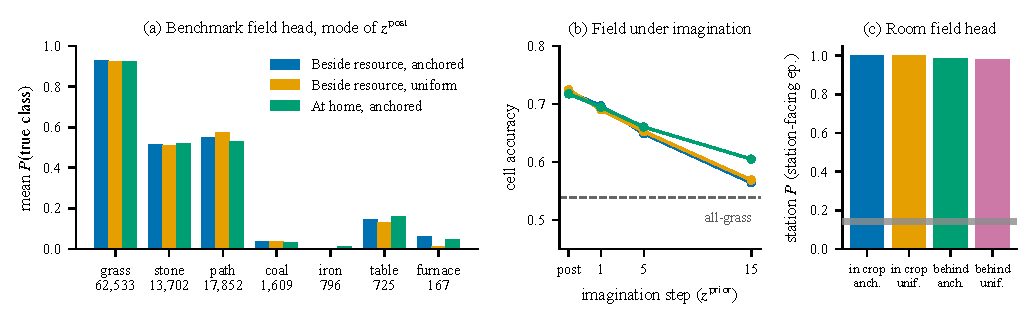
\includegraphics[width=\linewidth]{field_head.pdf}
  \caption{(a) Mean probability of the true class per material on the benchmark, with the number of probe cells under each label. (b) Cell accuracy of the field decoded from the posterior (``post'') and from the mode of $\zprior$ after 1, 5, and 15 imagined steps, against predicting grass everywhere (dashed). (c) In the room, the probability of the station on the station cells of a station-facing demonstration, for each of the four models; the gray band is the range of the benchmark's crafting-table probability from panel (a).}
  \label{fig:field}
\end{figure}

\paragraph{Under imagination.}
The actor is trained on the field decoded from $\zprior$, so the relevant question is what survives a rollout.
\Cref{fig:field}(b) shows that accuracy is about 70\% one step into imagination, then falls to 65--66\% at five steps and 56--61\% at fifteen, the length of an imagined training rollout, against the \FieldBaseline\% grass floor.
Stone and path recall fall with it, while grass stays near 0.8, so by the end of the horizon the predicted field has drifted toward grass.
The station is not recovered: table recall is 0.08 at step 15 in all three runs (\cref{tab:prior} in \cref{app:extra}).
These rollout scores cover 3,465 cells per step, of which only 17--25 are table and 3--6 furnace, so the station recalls under imagination are coarse.
The decoded frames of these rollouts are dark and low in contrast (\cref{fig:openloop}); we read the field numbers, not the images.

\subsection{Room: the station is named}

In the room the same probe gives a different answer (\cref{fig:field}(c), \cref{tab:room-probe}).
All four models reach material accuracy 1.0 on both demonstrations, station recall 1.0, and no false station cells.
On the station-facing demonstration the models trained in that pose assign the station a mean probability of 1.000, and the models trained facing away assign 0.986 and 0.981.
Under imagination from the first frame of the hold, the field stays correct for 15 steps in the pose each model trained on.
The two models trained facing away still predict the station one step into an imagined station-facing hold and lose it by step five; the models trained facing the station keep it through step 15.
So in the room, but not on the benchmark, the latent states where the station is.

\section{The two conditions on the benchmark}
\label{sec:benchmark}

\Cref{tab:switches} gives the three matched runs.
The actor's own count of the iron pickaxe was two lives in every run.
None of the 15 held-out evaluations (five checkpoints in each of three runs, ten lives each) contained one.

\begin{table}[t]
  \centering
  \caption{The two conditions on the benchmark, 100k environment steps each, one seed each, all from the same starting checkpoint. \emph{Teacher finishes}: lives in which the demonstrator, given control after the actor crafted a stone pickaxe, went on to craft the iron pickaxe, out of all such handoffs. \emph{Actor, unaided}: lives with no handoff in which the actor crafted the iron pickaxe. \emph{Held-out}: iron pickaxes in ten actor-only lives at 0, 25k, 50k, 75k, and 100k steps.}
  \label{tab:switches}
  \small
  % Generated by paper/scripts/build_assets.py. Do not edit.
\begin{tabular}{l l r r r l}
\toprule
Station & Window & Lives & Teacher finishes & Actor, unaided & Held-out, per checkpoint \\
\midrule
beside resource & anchored & 444 & 23/60 & 2 & 0, 0, 0, 0, 0 (of 10) \\
beside resource & uniform & 443 & 44/121 & 2 & 0, 0, 0, 0, 0 (of 10) \\
at home & anchored & 463 & 23/114 & 2 & 0, 0, 0, 0, 0 (of 10) \\
\bottomrule
\end{tabular}

\end{table}

\paragraph{Anchoring the window did not change the actor's count.}
The anchored and uniform runs share a demonstrator and differ only in $\rho_A$.
Both ended with two unaided iron pickaxes, out of \BenchMTwoTwoFieldCraftActor{} and \BenchMTwoThreeUniformWindowActor{} actor lives.
Anchoring was introduced because, in an earlier short run with uniform windows only, the cloning loss had fallen from 0.247 to $7\times10^{-5}$ while the actor had made no iron pickaxe, and most demonstrator windows did not contain the craft (\cref{app:window}).
Forcing the craft into half of the demonstrator windows for a full run did not move the count.
The demonstrator's finish rate was similar in the two runs, 38\% and 36\%, so the two runs saw comparable demonstrations of the rare action.

\paragraph{Station placement changed the demonstrations, not the actor's count.}
With the station walked back to rather than placed beside the resource, the demonstrator finished 23 of 114 handoffs (20\%), against 23 of 60 and 44 of 121 (about 37\%) when it placed the station beside the resource.
Replay therefore held roughly half as many completed demonstrations per handoff.
The actor's count stayed at two.

\paragraph{The held-out lives are the clean measurement.}
During training, a handoff begins as soon as an actor life has a stone pickaxe, so most lives in which the actor could have gone on to the iron pickaxe were given to the demonstrator.
The training-time unaided count is therefore censored by design, and we do not read two lives in several hundred as a difference between conditions in either direction.
The six that did occur came in lives of 48 to 300 steps, at irregular points in training.
Held-out lives have no handoff.
At 100k steps the actor crafted the stone pickaxe in \BenchMTwoTwoFieldCraftHeldstonefinal{}, \BenchMTwoThreeUniformWindowHeldstonefinal{}, and \BenchMTwoFourWalkHomeHeldstonefinal{} of its ten held-out lives in the three runs, and the iron pickaxe in none.
So the actor reached the precondition on its own, and with no demonstrator to take over, it still did not perform the rare action.

\paragraph{What the benchmark runs show.}
Both conditions changed something upstream of the actor.
Anchoring changed which demonstration steps the cloning loss saw; station placement changed how often demonstrations contained the craft at all.
Neither changed the field head, which named the station with probability below 0.16 in every run (\cref{sec:latent}), and neither changed the actor's count.
Because the actor is trained on imagined rollouts in which the predicted field does not contain the station, it receives no imagined return for crafting beside it, whatever the demonstrations show; the cloning term, which does see the true field, is the only signal that does.
The benchmark runs cannot separate this explanation from others, such as the length and survival demands of a Crafter life before the craft is reachable.
The room removes those demands.

\section{The same model in a room}
\label{sec:room}

The room keeps the model family, the field head, the actor input, the cloning term, and both conditions, and removes everything else that makes the benchmark hard: there is one room, one station, no survival, and a successful episode can be four steps long.
Unlike on the benchmark, the station can be outside the image at the moment of the action itself (\cref{fig:room-crops}).

\begin{figure}[t]
  \centering
  \begin{subfigure}[t]{0.16\linewidth}
    \centering
    
\includegraphics[width=\linewidth]{room-crop-facing-station.png}
    \caption{Facing the station.}
  \end{subfigure}\hspace{1.5em}
  \begin{subfigure}[t]{0.16\linewidth}
    \centering
    
\includegraphics[width=\linewidth]{room-crop-facing-away.png}
    \caption{Facing away.}
  \end{subfigure}
  \caption{The $64\times64$ observation from the cell south of the station. Each tile is $16\times16$ pixels, one cell of the encoder's final feature map. (a) The station (orange) is in the nearest row. (b) The station is one cell behind the agent and absent from the image; \texttt{use} succeeds from here only in the behind-agent condition. These are environment frames, not reconstructions.}
  \label{fig:room-crops}
\end{figure}

\begin{table}[t]
  \centering
  \caption{The two conditions in the room, 8,000 environment steps each, one seed each. \emph{Teacher}: demonstrator episodes that scored. \emph{Actor \texttt{use}}: actor training episodes that scored, out of all actor episodes; \emph{last quarter} restricts this to the final quarter of training. \emph{Eval}: actor-only successes out of eight at about 2k, 4k, 6k, and 8k steps. \emph{Median length}: steps in a successful actor training episode; the demonstrator uses at step 52 (in crop) or 54 (behind agent).}
  \label{tab:room}
  \small
  % Generated by paper/scripts/build_assets.py. Do not edit.
\begin{tabular}{l l l r r l r}
\toprule
Station at \texttt{use} & Window & Teacher & Actor \texttt{use} & Last quarter & Eval (/8) & Median length \\
\midrule
in crop & anchored & 8/8 & 124/147 & 30/37 & 7, 7, 8, 8 & 36 \\
in crop & uniform & 8/8 & 85/110 & 25/28 & 5, 4, 6, 8 & 42 \\
behind agent & anchored & 8/8 & 185/190 & 48/48 & 8, 8, 8, 8 & 38 \\
behind agent & uniform & 8/8 & 130/138 & 35/35 & 7, 8, 8, 8 & 46 \\
\bottomrule
\end{tabular}

\end{table}

\begin{figure}[t]
  \centering
  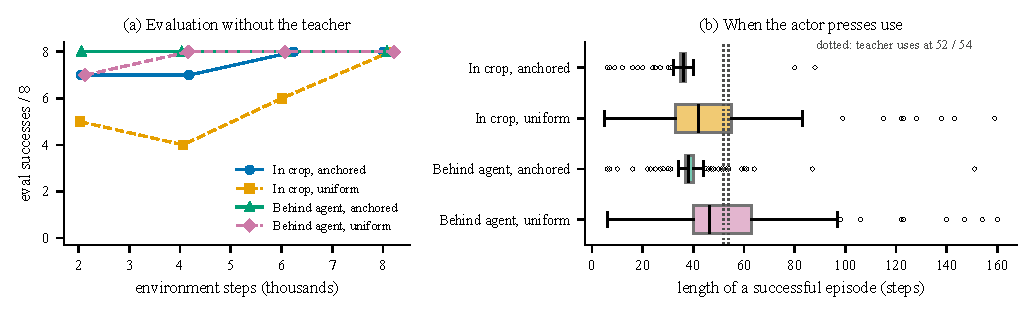
\includegraphics[width=\linewidth]{room_results.pdf}
  \caption{Room results, one seed per condition. (a) Actor-only evaluation successes out of eight. Solid lines are anchored windows, dashed lines uniform. (b) Length of every successful actor training episode. Dotted lines mark the demonstrator's \texttt{use} at step 52 (in crop) and 54 (behind agent).}
  \label{fig:room}
\end{figure}

\paragraph{The rare action is learned in every condition.}
\Cref{tab:room} and \cref{fig:room}(a) show that the actor learned \texttt{use} in all four runs.
Every run ended with eight of eight evaluation successes.
Every successful episode, in training and evaluation, was in the pose its condition requires, which the environment enforces.
Every failure was a 160-step timeout.
The behind-agent condition, in which the station is never in the image during the anchored window, was the more reliable of the two: \RoomOutAnchoredSuccess{} of \RoomOutAnchoredActor{} and \RoomOutUniformSuccess{} of \RoomOutUniformActor{} actor episodes scored, against \RoomInAnchoredSuccess{} of \RoomInAnchoredActor{} and \RoomInUniformSuccess{} of \RoomInUniformActor{} in crop, and its evaluations were at least seven of eight from the first one onward.
Removing the station from the image at the moment of the action did not prevent the action from being learned. That does not show the latent was supplying the station's location then. On real steps the field is the crop in front of the agent, so during the hold the station is in neither the image nor the field, and the facing-away probe's station cells are the four cells from the walk before the turn (\cref{tab:room-probe}). The latent does name the station on the frames where the station is visible (\cref{sec:latent}).

\paragraph{Anchoring changes when the actor acts, not whether.}
Uniform windows also learned the action in both poses.
What anchoring changed is the timing (\cref{fig:room}(b)).
With anchored windows, successful episodes cluster tightly: the median is \RoomInAnchoredMedian{} steps in crop and \RoomOutAnchoredMedian{} behind the agent, with 80\% of them between 31 and 38 steps and between 34 and 46 steps, respectively.
With uniform windows the medians are \RoomInUniformMedian{} and \RoomOutUniformMedian{}, and the middle 80\% spans 19 to 83 steps in crop and 28 to 84 behind the agent.
The in-crop uniform run was also the slowest to become reliable: its evaluations were 5, 4, and 6 of 8 before the final 8 of 8.
In every condition the actor acts well before the demonstrator's step 52 or 54, so it has not simply copied the length of the hold.

\paragraph{The room is not the benchmark.}
The room's \texttt{use} is one action from one cell in a fixed layout. The actor's first success came within the first 411 environment steps in every condition. Those steps count only the actor's interaction after training starts: the eight demonstrator episodes are collected before the loop and are not included.
The room shows that the recipe can produce the rare action in a layout where the station fills one encoder cell whenever it is in view, including a condition in which the station is behind the agent at the moment of acting. It does not show that the latent named the station during that hold.
It is not evidence that the recipe produces the benchmark's rare craft, which remained absent from every held-out life.

\section{Discussion}
\label{sec:discussion}

\paragraph{What the latent has to contain.}
A Dreamer-style actor learns from imagined rollouts, so an action can only acquire value in imagination if the imagined state distinguishes the situation in which the action pays off.
In \method{} we can read that distinction directly from the field head.
On the benchmark, the field head trained on the latent reached 72\% of cells, nearly all of the margin over the grass baseline came from terrain, and the station was named with probability 0.13--0.16 in the posterior and recall 0.08 after fifteen imagined steps.
In the room, where the station fills one encoder cell, it was named with probability above 0.98.
The actor learned the rare action where the station was named and did not where it was not, across both training conditions in each setting.
That co-occurrence is the paper's main observation.
It is consistent with the latent being the bottleneck, but two settings that differ in many ways cannot establish it.

\paragraph{What the benchmark runs do and do not show.}
They show that, at 100k steps from a shared checkpoint, neither anchoring the cloning window on the rare action nor placing the station beside the resource changed what the latent names or how often the actor performs the rare action.
They show that placement changed how often the demonstrations that enter replay contain the rare action.
They do not show that either condition is irrelevant in general: each is a single seed, the training-time unaided count is censored by the handoff, held-out evaluation is ten lives, and the benchmark's rare craft comes only after a long sequence of earlier achievements and survival.

\paragraph{Limitations.}
\begin{itemize}
  \item \emph{The actor reads the true field on real steps.} Every reported run gives the acting policy the environment's field, including at evaluation. The policy is trained on the predicted field in imagination, and the cloning term uses the true field. A run in which real steps read the predicted field would test whether the model alone can act, and we have not reported one.
  \item \emph{A second route on the benchmark.} In imagination, the benchmark's crafting actions are masked using the model's predicted inventory and neighborhood (\cref{sec:setup-crafter}). If that head does not predict the station nearby, the rare craft cannot be chosen in an imagined rollout at all. That would be a deficit of the same kind as the field head's, through a different head; we did not probe it. The room has no mask.
  \item \emph{One seed per configuration.} The differences between conditions that we report as absent are absent in one seed; the differences in the room's success timing are also from one seed.
  \item \emph{Small held-out sets.} Ten lives per benchmark checkpoint and eight episodes per room evaluation bound the resolution of every success rate we report.
  \item \emph{The room is easy.} It has a fixed layout and a single action. It isolates the station's visibility and the window, and nothing else from the benchmark.
  \item \emph{Model scale differs between settings.} The benchmark uses the XL configuration and the room a small one, chosen for the size of each observation's content; we do not vary scale within a setting.
\end{itemize}

\paragraph{Directions.}
Four experiments follow directly.
Probing the benchmark's neighborhood head, with the same protocol as the field head, would show whether the action mask removed the rare craft from imagined rollouts.
Running the actor on the predicted field at real steps would remove the privileged input and test the model alone.
Weighting the field loss toward rare classes, or raising the encoder's spatial resolution so a tile is no smaller than a latent cell, would test whether naming the station on the benchmark changes the actor's count.
Repeating the benchmark comparison over several seeds would turn the absence of an effect into an estimate of its size.

\section{Conclusion}
\label{sec:conclusion}

\method{} adds a local symbolic field head to a Dreamer world model, lets the actor read that field, and uses it to ask what the latent names.
On Crafter, the latent names terrain and not the crafting station, and neither anchoring demonstrations on the rare action nor placing the station beside the resource changed that or the actor's unaided count.
In a room where the station fills one encoder cell, the latent names it and the same recipe learns the rare action in every condition, including with the station behind the agent.
Probing the field a policy is trained on, rather than its reconstructions, is a direct way to see which of these two situations a world model is in.


\section*{Disclosure of AI assistance}
An AI coding and writing assistant was used to implement parts of the training and analysis code and to draft the text of this paper. The author designed the study, ran every training run, and checked every reported number against the logs. All numbers, tables, and plots are regenerated from those logs by the script described in \cref{app:repro}.

\bibliographystyle{plainnat}
\bibliography{refs}

\clearpage
\appendix
\section{Hyperparameters}
\label{app:hyper}

\begin{table}[h]
  \centering
  \caption{Hyperparameters. Both settings use one seed per run.}
  \label{tab:hyper}
  \small
  \begin{tabular}{l l l}
    \toprule
    & Benchmark (Crafter) & Room \\
    \midrule
    Encoder channels, residual blocks per stage & (96, 192, 384, 768), 2 & (32, 64, 128, 256), 1 \\
    Embedding size & 12{,}288 & 4{,}096 \\
    Deterministic state $h$; RSSM MLP width & 4{,}096; 1{,}024 & 512; 512 \\
    Stochastic state & $32\times32$ categorical & $32\times32$ categorical \\
    Decoder & mirrored, linear output & mirrored, linear output \\
    Head MLPs & 5 layers $\times$ 1{,}024 & 2 layers $\times$ 512 \\
    Field cells $C$, materials $M$, objects $O$ & 63, 13, 8 & 16, 4, 2 \\
    Field object weight $w$ & 4 & 4 \\
    Other heads & reward, continue, inventory, neighborhood & reward, continue \\
    Actor, critic MLPs & 5 layers $\times$ 1{,}024 & 2 layers $\times$ 256 \\
    Action unimix & 0.01 & 0.01 \\
    \midrule
    Environment steps & 100{,}000 & 8{,}000 \\
    Batch $\times$ sequence length $L$ & $8\times64$ & $8\times32$ \\
    Train ratio & 512 & 256 \\
    Imagination horizon $H$ & 15 & 8 \\
    Discount, $\lambda$ & 0.997, 0.95 & 0.997, 0.95 \\
    Entropy scale & $3\times10^{-4}$ & $3\times10^{-4}$ \\
    Learning rates (world model; actor, critic) & $10^{-4}$; $3\times10^{-5}$ & $10^{-4}$; $10^{-4}$ \\
    $\beta_{\mathrm{dyn}}$, $\beta_{\mathrm{rep}}$ & 0.5, 0.1 & 1.0, 0.5 \\
    Free nats (dynamics; representation) & 1; 1 & 0; 1 \\
    Precision & bf16 & bf16 \\
    \midrule
    Demonstrator fraction $\rho_T$ & 0.5 & 0.5 \\
    Anchored fraction $\rho_A$ & 0.5 or 0 & 0.5 or 0 \\
    Rare-action weight $\kappa$, cloning weight & 8, 1 & 8, 1 \\
    Rare-action set $\rareset$ & place furnace, iron pickaxe, iron sword & \texttt{use} \\
    Demonstrator episodes & 32 at start ($\le$800 steps), 8 per 25k & 8 at start \\
    Handoff & after stone pickaxe, ends 32 steps after craft & none \\
    Evaluation & 10 lives every 25k & 8 episodes every 2k \\
    Episode cap & 10{,}000 & 160 \\
    \bottomrule
  \end{tabular}
\end{table}

The benchmark run's KL scales follow the DreamerV3 paper; the room's size configuration used the larger scales listed and no floor on the dynamics term.
We did not tune either setting's world-model hyperparameters for this paper.

\section{Identifiability notes}
\label{app:identifiability}

\subsection{A reconstruction path that skips the posterior}
\label{app:bypass}

An earlier version of our world model had a second decoder that reconstructed the frame from the encoder embedding $e_t$, alongside the decoder on $[h_t,\zpost_t]$, and the decoder on $[h_t, \zpost_t]$ was trained through a frozen copy of its weights.
The two paths share the encoder and the optimizer.
The embedding decoder became a plain autoencoder: its reconstructions showed terrain and parts of the inventory, while reconstructions from $[h_t,\zpost_t]$ stayed close to a mean grass frame.
At 12k steps the reconstruction error was about 0.032 (mean absolute) through the posterior and 0.027 through the bypass, and the summed loss looked healthy.
Several fixes that targeted the posterior path (more decoder capacity, a spatial posterior, extra reconstruction terms on small regions) were each locally plausible given that graph and did not help.
We removed the second path and trained the single decoder with live weights. At 50k steps the posterior reconstruction error was 0.0095, and the agent, trees, and inventory appeared in posterior reconstructions. That 50k figure is not a matched before-and-after against the 0.032 at 12k: the graph and the training length both changed, and we did not record the fixed graph at 12k steps. What the 12k checkpoint shows is that the bypass could pay the pixel loss about as well as the posterior path.
The general point is that any reconstruction path that does not pass through $\zpost_t$ lets the optimizer pay the pixel loss without putting information into the latent, so a latent probe is only meaningful on a graph without one.

\subsection{Tile size and latent cell size}
\label{app:geometry}

Crafter draws its $9\times7$ local view in 7-pixel tiles above a two-row inventory strip.
A four-stage stride-2 encoder reduces the $64\times64$ frame to a $4\times4$ map, so one latent cell covers $16\times16$ pixels, more than two tiles in each direction.
A decoder that upsamples with nearest-neighbor interpolation cannot place content within a cell: in a capacity test overfitting eight frames, a sub-pixel convolution decoder \citep{shi2016subpixel} reached 0.0076 mean absolute error on the inventory strip, against 0.0487 for nearest-neighbor upsampling.
Even with a capable decoder, a reconstruction that is sharp on average does not imply that the latent states which material occupies a particular tile, because the per-pixel loss is dominated by large uniform regions.
The field head makes that statement explicit and measurable.
The room's tiles are 16 pixels, so each tile is exactly one latent cell.
Transformer world models that tokenize Craftax-Classic frames as one token per 7-pixel tile avoid the mismatch by construction \citep{dedieu2025improving}.

\subsection{A cloning loss that never sees the rare action}
\label{app:window}

In an earlier short run with uniform windows only, the cloning loss fell from 0.247 at 256 training steps to $7\times10^{-5}$ by 20,224 environment steps, while the actor made no iron pickaxe in 94 lives.
Of the 32 demonstrator lives in replay, 22 contained the craft, around steps 170--245 of lives that were often 200--800 steps long.
Exactly one start position makes a 64-step window end on the craft. About 64 of several hundred possible starts produce a window that contains it, so a uniform draw contains it only a few percent of the time, and the averaged loss is indifferent to it.
This motivated anchored windows and the weight $\kappa$.
Over a full 100k-step run, anchoring did not change the actor's behavior (\cref{sec:benchmark}).

\subsection{Demonstrations injected on the collection environment}
\label{app:inject}

Every 25k environment steps, the benchmark loop adds eight new demonstrator episodes to replay.
In our implementation the demonstrator played them on the same environment instance that the actor's collector was using, while the actor's current life was still open.
When the injection returned, the actor's open life resumed inside the last demonstrator episode's world, with that episode's inventory and achievement counters.
If that demonstrator had already crafted the iron pickaxe, the handoff rule (stone pickaxe and no iron pickaxe) never fired, and the life was logged as an unassisted iron pickaxe.

The logs show the signature exactly.
Before we found the leak, the three runs appeared to contain two unassisted iron pickaxes each, and the starting checkpoint's run appeared to contain \StartSpanningRare{}.
Every one of these lives started before an injection and ended within 136 environment steps after it, and they include lives of \BenchSpanningShortest{} and 19 steps that are credited with coal, a furnace, iron, and the iron pickaxe.
The only iron swords and diamonds in the three runs' training logs also sit on these lives, although the handoff demonstrator never made either.
We reproduced the mechanism with the environment alone: a random life with no achievements, followed by an injection on the same instance and a single further step, reports the iron pickaxe and eighteen other achievements.

We therefore exclude, from every benchmark count, the training lives that span an injection: three per run (one per injection) and \StartSpanning{} in the starting checkpoint's run.
With them excluded, the actor's unaided iron-pickaxe count is zero in all four runs.
One excluded life in the at-home run had been handed off after it inherited a stone pickaxe, which is why that run's handoff count is 113.
Held-out evaluations use a separate environment instance and are unaffected.
The general point is that, when demonstrations and agent experience share an environment object, an episode boundary on one side need not be an episode boundary on the other, and success counts can silently absorb the demonstrator's achievements.

\section{Accounting for demonstrator lives}
\label{app:accounting}

On the benchmark, the training log records every life with the achievements it unlocked and, for lives the demonstrator took over, an \emph{assisted} flag.
A life's stone pickaxe is always crafted by the actor, because the handoff begins only after it.
Everything after the handoff is the demonstrator's.
We count a life as the actor's only if it has no assisted flag and was not open during a demonstrator injection (\cref{app:inject}).
A Crafter score computed over all lives would include achievements the demonstrator unlocked after handoffs, and we therefore do not report one as the method's score.

In the beside-resource anchored run, the \BenchMTwoTwoFieldCraftLives{} counted lives contain 84 assisted lives, of which 60 are stone-pickaxe handoffs.
The other 24 form one block between 61,472 and 66,768 environment steps, when a rule that handed over lives at low health was briefly enabled; none has a stone pickaxe, they are excluded from both the handoff denominator and the actor's lives, and the rule was disabled for the other two runs.
In the other two runs every assisted life is a stone-pickaxe handoff.
Several lives can end within one logging interval and share an environment-step stamp; each log row is a distinct life.

In the room there is no handoff and no injection.
Demonstrator episodes are the eight collected before training, all of which scored, and every other episode is the actor's.

\section{Additional results}
\label{app:extra}

\begin{table}[h]
  \centering
  \caption{Benchmark field under imagination. The posterior row repeats \cref{tab:field} as recall. Prior rows decode the field from the mode of $\zprior$ after $k$ imagined steps from the posterior mode at every 32nd probe step, given the demonstrator's actions; each row scores 3,465 cells, of which 17--25 are table and 3--6 furnace. The 0.33 furnace recall is two of six cells.}
  \label{tab:prior}
  \small
  % Generated by paper/scripts/build_assets.py. Do not edit.
\begin{tabular}{l l r r r r r r }
\toprule
 & & & \multicolumn{5}{c}{recall} \\
\cmidrule(lr){4-8}
Run & Source & Acc. & grass & stone & path & table & furnace \\
\midrule
Beside resource, anchored & posterior & 72.1\% & 0.93 & 0.53 & 0.55 & 0.15 & 0.06 \\
 & prior, step 1 & 69.7\% & 0.91 & 0.50 & 0.51 & 0.35 & 0.20 \\
 & prior, step 5 & 64.9\% & 0.89 & 0.38 & 0.44 & 0.18 & 0.00 \\
 & prior, step 15 & 56.4\% & 0.80 & 0.33 & 0.39 & 0.08 & 0.00 \\
\midrule
Beside resource, uniform & posterior & 72.4\% & 0.93 & 0.52 & 0.59 & 0.13 & 0.01 \\
 & prior, step 1 & 69.0\% & 0.91 & 0.49 & 0.52 & 0.24 & 0.00 \\
 & prior, step 5 & 65.3\% & 0.88 & 0.39 & 0.50 & 0.27 & 0.00 \\
 & prior, step 15 & 56.9\% & 0.79 & 0.38 & 0.39 & 0.08 & 0.33 \\
\midrule
At home, anchored & posterior & 71.7\% & 0.93 & 0.53 & 0.54 & 0.16 & 0.05 \\
 & prior, step 1 & 69.5\% & 0.91 & 0.52 & 0.50 & 0.29 & 0.00 \\
 & prior, step 5 & 66.0\% & 0.89 & 0.50 & 0.42 & 0.27 & 0.00 \\
 & prior, step 15 & 60.5\% & 0.85 & 0.41 & 0.43 & 0.08 & 0.00 \\
\bottomrule
\end{tabular}

\end{table}

\begin{table}[h]
  \centering
  \caption{Room field head from the mode of $\zpost$, one correct demonstrator episode per pose (52 station cells when facing, 4 when facing away, from the walk before the turn). \emph{False}: fraction of non-station cells predicted as station.}
  \label{tab:room-probe}
  \small
  % Generated by paper/scripts/build_assets.py. Do not edit.
\begin{tabular}{l r r r r r r}
\toprule
 & \multicolumn{3}{c}{station-facing episode} & \multicolumn{3}{c}{facing-away episode} \\
\cmidrule(lr){2-4}\cmidrule(lr){5-7}
Trained on & recall & $P$ & false & recall & $P$ & false \\
\midrule
In crop, anchored & 1.00 & 1.000 & 0.00 & 1.00 & 1.000 & 0.00 \\
In crop, uniform & 1.00 & 1.000 & 0.00 & 1.00 & 1.000 & 0.00 \\
Behind agent, anchored & 1.00 & 0.986 & 0.00 & 1.00 & 0.999 & 0.00 \\
Behind agent, uniform & 1.00 & 0.981 & 0.00 & 1.00 & 0.999 & 0.00 \\
\bottomrule
\end{tabular}

\end{table}

\begin{figure}[h]
  \centering
  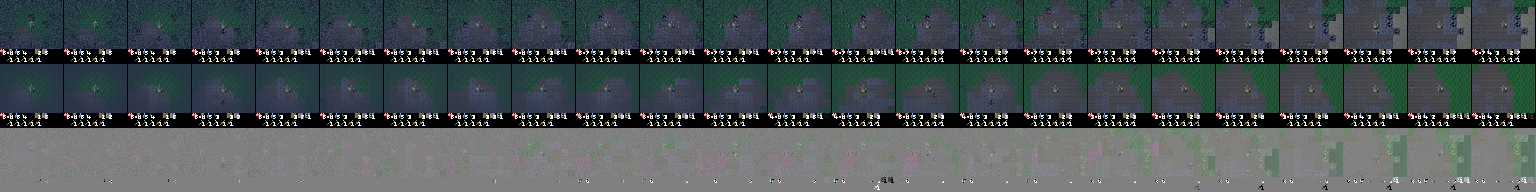
\includegraphics[width=\linewidth]{field-open-loop-station-inside.png}
  \caption{Open-loop prediction from the beside-resource anchored run at 100k steps. Rows: environment frames, model frames (the first eight columns reconstruct from the posterior, the rest are imagined from the prior given the recorded actions), and absolute error. The segment is the probe window with the most station cells; the environment frames themselves are dark, as at night in Crafter's day cycle. The other two runs give visually similar strips. We report the field head, not these images.}
  \label{fig:openloop}
\end{figure}

\section{Reproducibility}
\label{app:repro}

Every number, table, and plot in this paper is produced from the training logs and probe summaries by one script, which reads the per-life and per-episode logs, applies the exclusion rule of \cref{app:inject}, recounts the actor's and demonstrator's lives, and writes the tables and figures.
\Cref{fig:example} comes from a separate inference-only script that runs one benchmark checkpoint over a stored probe episode, and the injection leak is reproduced by a script that uses the environment alone.
The repository contains the world model, the field head, the room environment and demonstrator, the training loops for both settings, the probe scripts, and the configuration files for all seven runs.
At the logged rate of 0.65--1.05 environment steps per second, a benchmark run took one to two days on one 16\,GB GPU; a room run took under an hour.


\end{document}
